%texlive-2008
\documentclass[a4paper,12pt]{article}
\usepackage{usu8}
\usepackage{graphicx}

\begin{document}
\title{О способах и технологиях расширения языков программирования}
\author{Артем Мелентьев}
\maketitle

\begin{abstract}
В работе приведено сравнение различных средств для расширения как
синтаксических, так и семантических возможностей языков программирования (в
основном Java). Также приведены способы создания таких средств.
\end{abstract}

\tableofcontents

\section{Введение}

В процессе разработки ПО, как правило, используются универсальные языки
программирования, возможностей которых зачастую не хватает для многих областей.
Естественным образом появляется задача подгонки возможностей языка под
конкретную предметную область. Отсюда возникает задача исследования расширений
языков программирования. Задачами данной работы являются, во первых,
исследование наработок данной области, и во вторых составить возможный план
создания такого сорта расширяемого компилятора.

История расширяемых языков программирования начинается в 60ых годах с работ о
макросах и компиляторах компиляторов. Область была очень активна и все хотели
создать действительно расширяемый язык программирования. В то время
представлен проект расширяемого языка программирования Simula. Но его
расширяемость вополтить так и не удалось. Интерес к области стал снижатся в 70ых
годах. Одним из объяснений является черезмерная сложность создания расширений.
Активный интерес к области появляется в начале 21 века. Изза всеобщей
компьютеризации многим областям необходимы были специальные языки
программирования, а развитие методов программирования позволило создавать
расширяемые языки. Подробней про историю расширяемых языков можно прочитать в
основной части.

Тем не менее действительно расширяемые языки все еще очень трудно реализуемы.
Помимо обеспечения расширяемости, трудности возникают и с их отладкой,
совместимостью расширений. Также некоторые опасаются, что расширяемые языки
затруднят взаимодействие программистов, т.к. будут поощрять созданий
индивидуальных расширений ``под себя'', что каждый будет писать на своем
диалекте языка, несовместимом с диалектом другого.

Некоторые, как например SQLJ, создают одиночные расширения базового языка. 
которое не позволяет дальнейших расширений (по крайней мере внешне). Такие
расширения в работе также исследуются.

В развивающихся языках тоже можно проследить расширения. Так например в язык C\#
в каждой версии добавляется множество синтаксических расширений, наиболее
значительные из них в версии 3.0. Но их сложно оценивать с точки зрения
создания расширений, т.к. это внутренние расширения, и они сильно связаны с
языком. В большинстве языков программирования нет системы создания расширений и
для создания расширений требуется отличное знание устройства языка.

В отличие от C\#, Java более консервативнее и синтаксически меньше. Java
специально создавалась минимальной для облегчения взаимодействия программистов.
Отчасти благодоря этому Java сейчас наиболее популярный язык программирования
\cite{tiobe}. Как следствие большого сообщества и большей необходимости
расширений, у языка Java гораздо больше внешних расширений и исследований в этой области чем у C\#.
Поэтому в данной работе в основном исследуются расширения языка Java и смежных
языков. Автор также не скрывает большого опыта работы с ним и личного
предпочтения.

Для создания расширений с нуля используются множество инструментов, которые
облегчают их создание: генераторы лексеров, генераторы парсеров, компиляторы
компиляторов, различные вспомогательные блибиотеки, средства связи со средой
разработки и прочее. Все это будет рассмотрено в главе 3.

Прежде чем начать исследование, определимся с определениями, схемой компилятора
и возможными местами расширений.

\subsection{Схема компилятора}

\begin{center}
 Примерная структура компилятора
 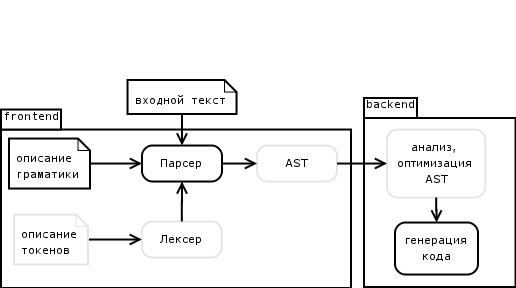
\includegraphics[scale=0.6]{img/compiler.png}
\end{center}

\subsection{Классификация}

Тем не менее область продолжает развиватся.
Из разных областей пришли понятия, которые нередко пересекаются смыслом.
Из языка Lisp пришло понятие языково-ориентированное программирование
Также оформилось понятие язык предметной области (Domain Specific Language, DSL), который бывает 
внутренним (встроенным, embeded) или внешним. Внутренний DSL реализуется внутри базового языка
посредством его синтаксических конструкций. Ярким примером внутреннего DSL является библиотека
CLOS (Common Lisp Object System) в яызке Lisp, которая добавляет в язык
возможности объектно-ориентированного программирования.


Расширения языка можно условно подразделить на семантические и синтаксические.
Семантические расширения меняют поведение программы каким-либо внешним образом
(например системы трансформации программ), а синтаксические - изменяют синтаксис
языка (пример - препроцессоры, макросы).

\section{Основная часть}

\subsection{История}
Область расширяемых языков программирования впервые появилась в 60ых годах
\cite{hist69}. Первая научная работа - ``Макросы для высокоуровневых языков
программирования'' принадлежит Дугласу Маклрою (M. Douglas Mcllroy's)
\cite{macro60}. Другие ранние описания принципа расширяемости приводятся в
статье Брукера и Мориса про компилятор компиляторов \cite{cc60}.
Пик движения отмечен двумя академическими симпозиумами, в 1969 \cite{proc69} и 1971
\cite{proc71}. Обзорная статья по данной области была написана в 1975 году
Томасом Стандишом \cite{Stan75}, после чего интерес к области начал пропадать.
Но интерес к области резко возрастает в 21ом веке \cite{Ext2105}.

\subsubsection{Характеристика раннего движения}

Расширяемый язык программирования состоит из простого базового языка и
метаязыка, способного изменять базовый язык. Расширенный язык получается
модификациями базового языка с помощью метаязыка. Большинство техник расширений
языка в то время были макроподстановками. Тем не менее модификации грамматик 
также исследовались, и в результате появились адаптивные грамматики, способные
изменять свой синтаксис прямо во время выполнения. Про них подробнее будет 
рассказано ниже. Сообщестно языка Lisp оставалось отделенным от сообщества
исследователей расширяемых языков, видимо потому что, как один исследователь
заметил, \cite{harr60}
\begin{quote}
любой язык программирования, в котором программа и данные существенно
неразличимы, может считаться расширяемым языком. \ldots это легко можно увидеть
из того факта, что Lisp использовался как расширяемый язык многие годы
\end{quote}
На конференции 1969 года был представлен Simula как расширяемый язык
программирования.

Стандиш описал три класса расширений языка, которые он назвал пересказ,
ортосказ и метасказ.
\begin{itemize}
  \item Пересказ (paraphrase) добавляет новые возможности, сводя их к уже
  имеющемуся. В качестве примера можно привести макроподстановки, которые в
  конечном счете разворачиваются в конструкции базового языка.
  \item Ортофраз (Orthophrase) добавляет возможности, невыразимые в базовом
  языке, такие как например добавление системы ввода-вывода к языку, не имеющему оной. Таким
  образом, ортофраз-расширение должно быть написано на другом языке. Из
  современных понятий близким аналогом является понятие plug-in.
  \item Метафраз (Metaphrase) модифицирует интерпретацию существующих элементов
  языка, и таким образом, выражения разбираются по новому. Оно соответсвует современному
  понятию рефлекции.
\end{itemize}

\subsubsection{Смерть раннего движения}

Стандиш аргументировал неудачу движения сложностью программирования последующих
расширений. Обычный программист может создать некое расширение вокруг базового
языка, но если второе расширение будет создано вокруг первого, то программисту
нужно быть близко знакомым и с базовым языком, и с первым расширением. Третье
расширение будет требовать еще больше знаний и так далее. Следует заметить, что
отделение программиста от низкоуровневых деталей - это цель движения
абстракции, которое вытеснило движение расширяемости в то время.

\subsection{Совмененное состояние}

В современном смысле, система, поддерживающая расширяемое программирование,
предоставляет все нижеперечисленные возможности:

\subsubsection{Расширяемый синтаксис}

TODO


Расширения компилятора можно условно подразделить на синтаксические и
семантические. Синтаксические расширения добавляют новые синтаксические
конструкции в язык. Пример – enum, generics в Java 1.5. Семантические
расширения, в отличие от синтаксических, просто меняют поведение кода, без
введения новых синтаксических конструкций. Примером семантических расширений
является аспектно-ориентированное программирование (АОП), которое будет
рассмотрено в дальнейшем.

\subsection{Семантические расширения}

Семантические расширения меняют поведение программы каким-либо внешним образом.

\subsubsection{Метапрограммирование}
Метапрограммирование — создание программ, которые создают другие программы как
результат своей работы (либо — частный случай — изменяющие или дополняющие себя
во время выполнения).

Метапрограммирование разделяется на 2 направления: на стадии
компиляции (генерация кода) и на стадии выполнения (самомодифицирующийся код).

Первое направление позволяет получить программу при меньших затратах времени и
усилий, чем если бы программист писал её вручную. Второе — расширяет
возможности программиста.

TODO: Meta Object Protocol

\subsubsection{Аспектно-ориентированное программирование}
Аспектно-ориентированное программирование (АОП) — парадигма программирования,
основанная на идее разделения функциональности, особенно сквозной
функциональности, для улучшения разбиения программы на модули.

Существующие парадигмы программирования, такие как процедурное программирование
и объектно-ориентированное программирование, предоставляют некоторые способы
для разделения и выделения функциональности, например, функции, объекты,
классы, пакеты, но некоторую функциональность с помощью предложенных методов
невозможно выделить в отдельные сущности. Такую функциональность называют
сквозной, так как её реализация разбросана по различным модулям программы.
Сквозная функциональность приводит к рассредоточенному и запутанному коду.
Запутанным называется такой код, в котором одновременно реализована различная
функциональность.

Трассировка — типичный пример сквозной функциональности. Другие примеры:
контрактное программирование, в частности проверка пред- и пост-условий,
обработка ошибок, реализация систем безопасности. Если рассматривать программу
написанную с помощью ООП, то любая функциональность, по которой не происходила
декомпозиция программы, является сквозной.

Все языки АОП предоставляют способы для выделения сквозной функциональности в
отдельную сущность. Различие между ними заключается в удобстве, безопасности и
области применения средств, которые они предоставляют. Наиболее популярный на
данный момент язык АОП — AspectJ. Используемые в нем понятия распространились
на большинство языков АОП.

Основные понятия AspectJ:
\begin{itemize}
 \item Точка выполнения (англ. JoinPoint) — определенная точка выполнения программы.
 \item Срез (англ. PointCut) — набор точек выполнения программы.
 \item Применение (англ. Advice) — состоит из условий применения и реализации
 функциональности. Условия применения определяют до, после или вместо какого
 среза надо вставить требуемую функциональность.  
 \item Аспект (англ. Aspect) — модуль AspectJ.
 \item Представление (англ. Introduction) — метод изменения структуры класса
 путем введения новых полей и методов, а также изменения иерархии наследования.
\end{itemize}

АОП не применяется сама по себе, а только в контексте какой-нибудь другой
парадигмы, чаще всего ООП.

АОП можно рассматривать как вариант метапрограммирования при компиляции.
Обычно аспекты описываются расширенным базовым языком, поэтому такое АОП можно
рассматривать и как синтаксическое расширение. Но существуют и реализации АОП
обходящиеся только средствами языка (например с помощью аннотаций Java5).

\subsubsection{Макросы}
 Макрос (от англ. macros, мн.ч. от macro) — программный объект, при обработке
«развертывающийся» в последовательность действий или команд.

Макросы по отношению к языку можно разделить на внешние и внутренние.
Внешние макросы не связаны с языком, и не имеют доступа к контексту применения.
Пример внешних макросов - препроцессор языка C, который реализован внешней
утилитой (cpp, The C PreProcessor) и никак не связан с языком.

Внутренние макросы, в отличие внешних, имеют доступ к контексту применения, и
поэтому обладают гораздо большей выразительной способностью. Как следствие,
внутренние макросы тесно связаны с языком. При применении они могут имеют
доступ к дереву разбора и могут изменять его.

Наиболее мощными внутренними макросами обладают языки семейства lisp
(lisp, scheme). Языки nemerle и boo также обладает мощной встроенной системой
макросов, с помощью которых можно даже добавлять новые синтаксические
конструкции в язык. Для языка Java существует система внутренних макросов Java
Syntactic Extender, которая будет рассмотрена ниже.

\subsubsection{Eclipse Java AST}
Используется в Eclipse IDE для проведения рефакторингов и в Eclipse Java
Compiler(ejc).

TODO

\subsubsection{Системы трансформации программ}
Техники трансформации программ используются во многих сферах: от генерации
программ, оптимизации и рефакторинга до обратной разработки и генерации
документации.
Данная область является, наверное, самой старой. Многие теории, инструменты и
приложения в этой области разработаны более 30 лет назад.
В связи большим возрастом области, в ней сформировались некоторые стандарты.
В первую очередь это SDF - syntax definition formalism, формат файлов для
описания грамматик контекстно-свободных языков. форматом SDF пользуются
большинство систем трансформации.
Кроме того проект SDF предоставляет стандартный генератор парсеров класса SGLR
(Scanerless Generalized Left-to-right Rightmost derivation parser, иногда
называемый параллельным парсером, расширение LR парсера, для поддержки
недетерминированных и неоднозначных грамматик; алгоритмическая сложность разбора
= $O(n^3)$; при отсутствии неопределенностей - $O(n)$).

Некоторые системы трансформации:
\begin{itemize}
  \item Stratego/XT
  \item ASF+SDF Meta Environment
  \item TermWare
\end{itemize}

\subsection{Синтаксические расширения}
Как уже было сказано, синтаксическое расширение добавляет в язык новые
синтаксические конструкции, и связывает с ними какую-либо семантику.

\subsubsection{Java Syntactic Extender}
Java Syntactic Extender (JSE) - расширение языка Java, позволяющее добавлять в
язык новые синтаксические конструкции. Оно основано на системе макросов Dylan с
учетом специфики языка Java. Расширения могут быть реализованы
непосредственно на Java без каких-либо ограничений. JSE - это
препроцессор языка Java, который разворачивает макросы.

JSE использует парсер языка Java с макросами, основанный на генераторе парсеров
ANTLR. Парсер строит специальное дерево разбора, которое в JSE называется
Skeleton Syntax Tree (SST). В дальнейшем макросы явно или неявно манипулируют
именно SST.

Сами макросы представляют из себя обычные классы Java, которые, имея доступ к
SST, разворачивают вызов макроса во что угодно. После применения всех макросов,
SST преобразуется обратно в текст для компиляции стандартным компилятором.

Недостатки:
\begin{itemize}
 \item не учитывается область видимости, возможен конфликт имен
 \item мало контекстной информации
 \item проект заброшен
\end{itemize}

\subsubsection{OJ}
OJ (бывшая OpenJava). Добавляет MetaObject Protocol в Java.
Позволяет изменять, создавать классы во время выполнения.
Проект заброшен. Возможно АОП оказалось более перспективным направлением.

\subsection{Расширяемые компиляторы}
\subsubsection{Polyglot}
Polyglot - расширяемый текстовый преобразователь Java программ (транслятор из
Java в Java). Polyglot состоит из базового компилятора jlc и его расширений.
Компилятор jlc - полноценный Java фронтенд. Он разбирает и проводит
семантический анализ исходного кода. Компилятор генерирует исходный Java код.
Таком образом базовый компилятор не производит трансляции в байт-код, в отличие
от стандартного компилятора Java.

Языковые расширения реализуются поверх базового компилятора путем расширения
конкретного и абстрактного синтаксиса, системы типов и определения новых
трансформаций кода. В результате получается абстрактное синтаксическое дерево
(AST), которое преобразуется в исходный код на Java и компилируется стандартным
компилятором javac.

\begin{center}
Частичное дерево языков, основанных на Polyglot:
 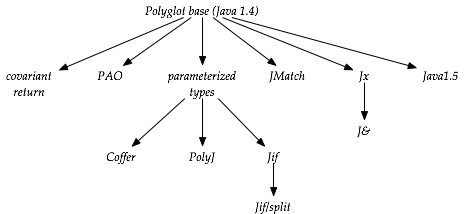
\includegraphics[scale=0.6]{img/polyglot-tree.png}
\end{center}

В Polyglot используется Polyglot Parser Generator~(PPG) - собственный генератор
парсеров на основе JavaCUP.

Polyglot - пример наиболее популярного подхода к созданию расширений языка:
сведение конструкций нового языка к конструкциям на базовом языке. Но, в
отличие от других подобных проектов, Polyglot смог собрать вокруг себя большое
сообщество, что привело к появлению многих расширений языка Java на его основе.
К сожалению, в последнее время активность проекта упала, и некоторые проекты
(например Soot, Aspect Bench Compiller(abc)) переходят на использование более
перспективного проекта JastAdd.

\subsubsection{JastAddJ}
Фактически JastAdd - это специальное расширение языка AspectJ для создания
трансляторов и семантических анализаторов. JastAdd позволяет сделать из
обычного синтаксического дерева (AST) атрибутную грамматику (а точнее
Rewritable Circular Reference Attributed Grammar, циклическая (допустимость
циклических ссылок) ссылочная атрибутная грамматика с возможностью перезаписи
узлов, ReCRAG) средствами АОП. JastAdd добавляет атрибуты, их расчет и
различные действия над атрибутной грамматикой прямо в классы AST. В результате
получаются расширенные классы AST с атрибутами. Компилятор записывается как
расчет атрибутов дерева. Компиляторы можно писать как в декларативном
(рекомендуется), так и в императивном стиле.

JastAddJ - расширяемый компилятор Java на основе JastAdd.
JastAddJ состоит из:

Java1.4 frontend - разбирает Java 1.4 код, создает AST и производит
статико-семантический анализ (соответствие типов и т.д.).

Java1.4 backend - расширение Java1.4 frontend. Генерирует стандартный байт-код
для JVM.

Java1.5 frontend - расширение Java1.4 frontend. Добавляет синтаксические
расширения Java 1.5 (generics, annotations, и пр.).

Java1.5 backend - расширение Java1.5 frontend и Java1.4 backend. генерирует
байт-код.

Компилятор JastAddJ проходит большинство тестов тестового комплекта Jacks,
больше чем другие компиляторы, включая javac, ejc, polyglot jlc, jikes. При
этом JastAddJ медленнее javac всего примерно в 3 раза и меньше всех по объему
исходного кода~\cite{JastAddJ}.

В отличие от Polyglot, сообщество JastAdd довольно мало, и количество
расширений не так велико. Несмотря на это JastAdd успешно используется в
некоторых проектах в качестве экспериментальной замены Polyglot. Стоит
заметить, что JastAdd абсолютно не совместим с Polyglot. У них разные принципы
и способы работы, но цель одна - создание расширяемых компиляторов.

\subsection{Расширяемые языки программирования}

\subsubsection{Lisp}
Функциональный язык Lisp (и его наследники scheme, common lisp и пр.) имеет
жесткий базовый синтаксис скобочных выражений. Остальное расширяемо функциями,
макросами, лямбда-исчислением и концепцией кода программы как данных.

\subsubsection{Boo}
Boo - объектно ориентированный статически типизируемый язык для платформы .NET
со схожим с Python синтаксисом и специально ориентированном на расширяемость
языка и компилятора. Как и в Nemerle, Boo позволяет определять синтаксические
макросы, рекурсивно разворачивающивающиеся базовые конструкции языка путем
манипуляций с синтаксическим деревом. Макросы, как и в Java Syntactic Extender,
представляются просто объектом языка. Когда при синтаксическом разборе разборе
встречается неизвестная синтаксическая структура, парсер Boo проверяет,
является ли она макросом, и если является, вызывает соответствующие методы у
класса макроса.

\begin{example}
Макрос ``with'' на Boo
\end{example}
\begin{verbatim}
import Boo.Lang.Compiler
import Boo.Lang.Compiler.Ast
import Boo.Lang.Compiler.Ast.Visitors

class WithMacro(AbstractAstMacro):
    private class NameExpander(DepthFirstTransformer):
        _inst as ReferenceExpression
        def constructor(inst as ReferenceExpression):
            _inst = inst
        override def OnReferenceExpression(node as ReferenceExpression):
            if node.Name.StartsWith('_'):
                // create the new member reference and set it up
                mre = MemberReferenceExpression(node.LexicalInfo)
                mre.Name = node.Name[1:]
                mre.Target = _inst.CloneNode()
                // replace the original reference in the AST
                // with the new member-reference
                ReplaceCurrentNode(mre)
    override def Expand(macro as MacroStatement) as Statement:
        assert 1 == macro.Arguments.Count
        assert macro.Arguments[0] isa ReferenceExpression
        inst = macro.Arguments[0] as ReferenceExpression
        // convert all _<ref> to inst.<ref>
        block = macro.Block
        ne = NameExpander(inst)
        ne.Visit(block)
        return block
\end{verbatim}
\begin{example}
Применение макроса ``with'' на Boo
\end{example}
\begin{verbatim}
with fooInstanceWithReallyLongName:
    _f1 = 100
    _f2 = "abc"
    _DoSomething()
\end{verbatim}

\subsubsection{Nemerle}
Nemerle — это гибридный язык высокого уровня для платформы .NET со статической
типизацией, органично сочетающий в себе возможности функционального и
объектно-ориентированного программирования. Синаксически похож на C\#, ML,
OCaml, Haskell. Главная особенность языка - это очень мощная система
метапрограммирования.

Ряд языковых средств кардинальным образом отличает Nemerle от C\#, Java, C++.
Это макросы и замыкания, причём в виде, более характерном для Lisp или других
функциональных языков, нежели для С++. Система макросов позволяет описывать на
Nemerle новые синтаксические конструкции и использовать их наравне со
встроенными. В действительности, большинство директивных управляющих
конструкций, в том числе операторы if, when, циклы всех видов, реализованы в
виде макросов стандартной библиотеки Nemerle.

Макросы представляют из себя описание синтаксиса и действий. В действиях
возможно применение квази-цитирования (преобразование кода в цитате в AST для
добавления в синтаксическое дерево). Макросы компилируются предварительно в
библиотеки .NET, и в дальнейшем используются при разборе исходного кода с
макросами. Также как и в Boo, макросы применяются только на подходящих, но
неизвестных базовому парсеру, синтаксических конструкциях.

\begin{example}
Макрос с квазицитированием на Nemerle
\end{example}
\begin{verbatim}
macro ReverseFor (i, begin, body) 
syntax ("ford", "(", i, ";", begin, ")", body)
{
  <[ for ($i = $begin; $i >= 0; $i--) $body ]>
}
\end{verbatim}

Система макросов nemerle считаются одной из самых мощных. Многие
синтаксические возможности языка, на самом деле являются макросами. С помощью
его макросов можно, например, реализовать внутренние языки предметной области,
частичные вычисления, некоторые возможности аспектно-ориентированного
программирования и прочее.

Nemerle имеет опциональную возможность использовать отступы как структуру
программы (identation based syntax), подобно тому как это сделано в языке
Python. Т.е. вместо использования скобок для обозначения блоков, можно
использовать символ табуляции для их оформления (т.е. так называемая
``лесенка'' задает структуру, а не наоборот). Это можно рассматривать как
пример расширения лексера в nemerle.

\subsubsection{Scala}
Scala — это, подобно Nemerle, гибридный язык программирования, спроектированный
кратким и типобезопасным для простого и быстрого программирования. В нем органично
сочетаются возможности функционального и объектно ориентированного
программирования. Основной целью разработки был язык, обладающий хорошей
поддержкой компонентного ПО.

Говорят, что Scala расширяемый язык. На самом деле, синтаксис Scala просто
настолько широк, что позволяет легко создавать EDSL (Embeded Domain Specific
Language, внутренние языки предметной области) на основе Scala. Этому
способствуют closures (анонимные функции, также известные как замыкания), обилие
``синтаксического сахара'' (то есть синтаксических сокращений, например:
``a+b'' вместо ``a.+(b)'') и функциональная природа языка.

TODO: XLR, XPS

\section{Средства создания компиляторов}

TODO
\begin{center}
 Примерная структура компилятора
 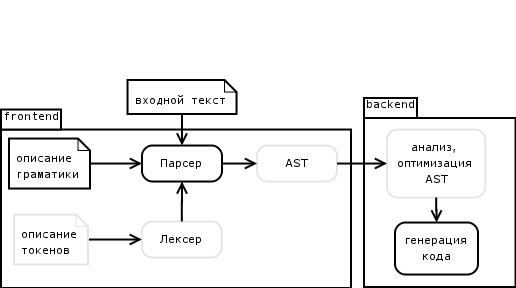
\includegraphics[scale=0.6]{img/compiler.png}
\end{center}

\subsection{Определения}
\begin{description}
  \item[Парсер] (Parser) -
    Синтаксический анализатор. Транслирует исходный текст в вид, который прост
    для программной обработки.
  \item[Компилятор компиляторов] (Compiler compiler) -
	Инструмент для создания парсера, интерпретатора или компилятора из формального
	описания языка.
  \item[Генератор парсеров] (Parser Generator) -
  	Наиболее ранняя и широко используемая форма компилятора компиляторов.
  	Создает парсер по описанию грамматики. 
  \item[лексема, токен] (lexem, token) - 
  	Атомарная единица парсера. например число, идентификатор. т.е. набор
  	символов по определенному признаку.
  \item[лексер, токенайзер] (lexer, tokenizer)-
  	Лексический анализатор. Выдает по строке символов, набор лексем. Некоторые
  	парсеры(yacc) могут требовать внешний лексер, а некоторые имеют встроенный.
  \item[Дерево разбора] (Parse Tree, Concrete Syntax Tree(CST)) -
  	корневое, помеченное дерево, представляющее синтаксическую структуру
  	исходного текста согласно какой-либо формальной грамматике. Внутренние узлы
  	дерева помечены нетерминалами грамматики, а листья дерева - терминалами.
  \item[Абстрактное синтаксическое дерево] (Abstract Syntax Tree(AST), или
  просто синтаксическое дерево) - Специальная разновидность дерева разбора,
  используемая в компиляторах. Отличается от дерева разбора отсутствием
  необязательных для семантики узлов (напр: запятые, скобки, ключевые слова) и
  некоторыми другими структурными отличиями.
\end{description}

\subsection{JetBrains MPS}
Meta Programming System - Среда разработки DSL и их интеграции в IDE Idea.
Позволяет с легкостью создать свой язык, редакторы и генераторы к нему.
Отличается от остальных инструментов тем, что хранит исходные файлы языка не в
простом текстовом формате, а хранит непосредственно синтаксическое дерево (в
XML). Таким образом парсеры и сериализаторы становятся не нужны, но
пользователь становится сильно зависимым от редактора.

Редактирование языка ведется путем создания типов и структуры синтаксического
дерева (структурного концепта в терминологии MPS). Далее для каждого нового типа
создается описание редактора, которое определяет то, как будет выглядеть часть
редактора языка для данного типа синтаксического дерева. Делается это путем
расстановки полей ввода и различных подписей. Редактор редакторов - одна из
сильнейших сторон MPS. Пользоваться им достаточно просто.

Генератор представляет из себя шаблон кода, который применяется к языку. В
результате может получится, например, интерпретатор языка на Java. Редактор
генераторов позволяет легко создавать сложные шаблоны с подстановками,
итерациями и пр.

MPS поддерживает множественное наследование языков. При этом просто происходит 
объединение всех типов синтаксического дерева всех языков. Благодаря хранению
исходных файлов в виде синтаксического дерева, снимается проблемы
множественного наследования, имеющиеся в других инструментах.

В MPS реализовано множество языков, в том числе сама Java, которая применяется
в редакторе генераторов. Пользоваться MPS новичкам очень просто. Но для хорошо
знакомых с языком, MPS может показаться слишком ограничивающим, т.к. не позволяет
свободное редактирование кода (ввод только в поля ввода). Поэтому MPS больше
подходит для создания небольших языков.

Большая часть исходного кода MPS открыта под лицензией Apache~2.0. Закрытой
является используемая в MPS часть IDE Idea, которая является коммерческим
продуктом.
На данный момент доступна версия 1.0beta2.

\begin{center}
Редактор редакторов MPS:
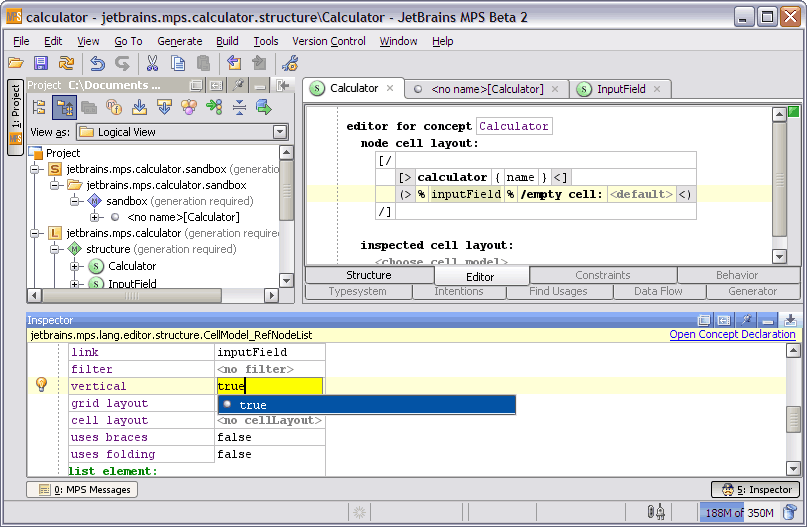
\includegraphics[scale=0.4]{img/mps.png}
\end{center}

\subsection{Textual Modeling Framework(TMF) Xtext}
Аналог MPS для IDE Eclipse.
Набор инструментов для создания внешних DSL и редактора к ним на основе Eclipse.
Основано на технологиях Eclipse Modeling Framework(EMF), Graphical Modeling
Framework(GMF), Model To Text (M2T), Eclipse Modeling Framework Technology
(EMFT). На текущий момент (0.7.0RC1) проект находится на стадии разработки
(Eclipse incubation). Планируется интеграция в следующую версию Eclipse 3.5
Galileo.

В Xtext, в отличие от MPS, исходные файлы хранятся в обычном текстовом формате.

Грамматика одновременно с моделью задается с помощью компактного и
выразительного языка, в форме, похожей на сильно расширенную EBNF.

Xtext по грамматике языка создает:
\begin{itemize}
  \item инкрементальный парсер и лексер, основанный на ANTLR (в разработке
  собственный генератор парсеров packrat)
  \item мета модель, основанная на Ecore.
  \item сериализатор, используемый для преобразования мета модели обратно в
  текстовую форму, с сохранением исходного форматирования 
  \item интеграцию языка в Eclipse IDE:
  \begin{itemize}
    \item подсветка синтаксиса
    \item навигация (F3, и т.п.)
    \item автодополнение кода (ctrl-space)
    \item outline view
    \item шаблоны кода
  \end{itemize}
\end{itemize}

В качестве языка для генераторов кода, в Xtext используется Xpand
(статически-типизируемый шаблонный язык)

\begin{example}
Пример описания языка в Xtext:
\end{example}
\begin{verbatim}
Model:
  (types+=Type)*;

Type:
  DataType | Entity;

DataType:
  "datatype" name=ID;

Entity:
  "entity" name=ID "{"
    (features+=Feature)* 
  "}";

Feature:
  type=[Type|ID] name=ID;   
\end{verbatim}

По мнению автора xtext хорошо подходит для создания малых языков предметной
области, но не для создания полноценных языков. 

\subsection{Eclipse IDE Meta-Tooling Platform}
Eclipse IMP - это набор инструментов для создания среды разработки для
произвольных языков.
Eclipse - это отличная среда для разработки на Java, но для
других языков программирования сделать подобную среду очень сложно. Цель
Eclipse IMP - упростить создание среды разработки на основе Eclipse для
произвольных языков.

В отличие от Xtext который ориентирован на небольшие языки предметной области
(DSL), IMP ориентирован на полноценные языки программирования. На основе IMP
были разработана среды для языков X10 и XJ, которые являются расширениями
языка Java.

Фактически IMP - это просто набор инструментов для создания сервисов к IDE для
разрабатываемого языка. В IMP интегрирован генератор парсеров LPG (ранее
известный как JikesPG), но возможно использование и других генераторов или
самописных парсеров.

Если компилятор генерирует Java файлы, IMP сможет даже их отлаживать благодаря
стандарту JSR-45~\cite{JSR45}. Для этого нужно в Java-файлы вставлять
комментарии вида ``//\#line'' для соответствия строк в исходном файле и сгенерированном по нему Java-файле.

IMP, LPG, X10, XJ - проекты компании IBM.

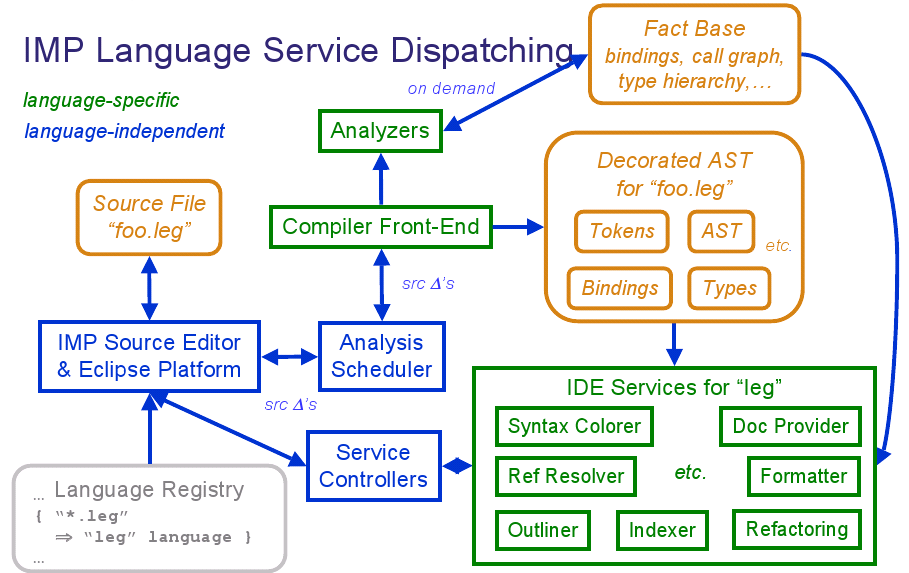
\includegraphics[scale=0.4]{img/imp.png}

\subsection{Генераторы парсеров}

\subsubsection{yacc}
\begin{description}
  \item[распознаваемый класс языков]: LALR(1)
  \item[целевые ЯП]: yacc: C; bison: C, C++; и др.
  \item[особенности]: стандартизован в POSIX P1003.2. требует внешнего лексера: lex, flex.
\end{description}
yacc — стандартный генератор парсеров в Unix-системах. Название является
сокращением от «Yet Another Compiler Compiler» («всего лишь ещё один генератор
компиляторов»). Yacc генерирует парсер на основе аналитической грамматики,
описанной в нотации BNF. На выходе yacc выдаётся код парсера на языке
программирования Си.

Yacc был разработан Стивеном Джонсоном (Stephen C. Johnson) в компании AT\&T
для операционной системы Unix. Позже были написаны совместимые версии
программы, такие как Berkeley Yacc, GNU bison, MKS yacc и Abraxas yacc
(обновлённый вариант AT\&T-версии с открытым исходным кодом также вошёл в
проект OpenSolaris от Sun). Каждый вариант предлагал незначительные улучшения и
дополнительные возможности по сравнению с оригиналом, но концепция осталась той
же. Yacc также был переписан на других языках, включая Ratfor, EFL, ML, Ada,
Java, C\# и Limbo.

Парсер, генерируемый с помощью yacc, требует использования лексического
анализатора. В качестве него в большинстве случаев испльзуется lex либо
flex. Стандарт IEEE POSIX P1003.2 определяет как функциональность так и
требования для lex и yacc.

\begin{example}
Пример калькулятора на yacc
\end{example}
\begin{verbatim}
..
line   : exp ';' '\n'       {printf ("result is %d\n", $1);}
        ;
exp    : term               {$$ = $1;}
        | exp '+' term      {$$ = $1 + $3;}
        | exp '-' term      {$$ = $1 - $3;}
        ;
term   : factor             {$$ = $1;}
        | term '*' factor   {$$ = $1 * $3;}
        | term '/' factor   {$$ = $1 / $3;}
        ;
factor : number             {$$ = $1;}
        | '(' exp ')'       {$$ = $2;}
        ;
number : digit              {$$ = $1;}
        | number digit      {$$ = $1*10 + $2;}
..
\end{verbatim}

Как видно из примера, описание грамматики для yacc состоит из правил вывода и
некоторых действий, выполняемых при обнаружении данного вывода.
Yacc генерирует С-файл с парсером, который выполняет указанные действия.
Таким образом сгенерированный парсер НЕ строит дерева разбора. Его нужно строить
самостоятельно в действиях описания грамматики.

\subsubsection{ANTLR}
\begin{description}
  \item[распознаваемый класс языков]: LL(*) (шире чем LALR(1))
  \item[целевые ЯП]: Java, C++, C\#, Python, Ruby
  \item[особенности]: наиболее мощный по возможностям. требует специальную
  библиотеку для работы сгенерированного парсера (runtime dependency)
\end{description}
ANTLR — буквально Another Tool For Language Recognition (Ещё Одно Средство
Распознавания Языков) — генератор парсеров, позволяющий автоматически создавать
программу-парсер(как и лексический анализатор) на одном из целевых языков
программирования(С++, Java, C\#, Python, Ruby) по описанию LL(*)-грамматики на
языке, близком к EBNF. Позволяет конструировать компиляторы, интерпретаторы,
трансляторы с различных формальных языков. Предоставляет удобные средства для
восстановления после ошибок и сообщения о них. ANTLR — продолжение PCCTS(Purdue
Compiler Construction Tool Set), который был разработан в 1989 г.

Основоположником проекта и его главным вдохновителем является проф. Теренс Парр
(Terence Parr) из Университета Сан-Франциско. ANTLR — проект с открытым
свободным кодом, версия 3.1 распространяется по лицензии BSD. Проект в
настоящее время активно развивается.

Создатели ANTLR утверждают, что многие преимущества при определении действий
для правил являются следствием того, что ANTLR осуществляет LL разбор, то есть
использует разбор сверху вниз, в отличие от yacc, bison, которые
используют разбор снизу вверх. LL(*) разбор проще в понимании и
диагностике ошибок чем LR(1). К тому же класс языков распознаваемых LL(*)
разбором шире чем LR(1). Кроме того ANTLR выгодно отличается от других наличием
визуальной среды разработки ANTLRWorks, позволяющей удобно создавать и
отлаживать грамматики: это многооконный редактор, поддерживающий подсветку
синтаксиса, автодополнение, визуальное отображение грамматик, строящееся в
реальном времени по мере ввода, отладчик, инструменты для рефакторинга и т. д.

ANTLR, также как и yacc, выполняет указанные действия для правил вывода.

\begin{example}
простейшая программа на ANTLR
\end{example}
\begin{verbatim}
grammar T;
//нетерминальные символы:
msg : 'name' ID ';' 
	{
		System.out.println("Hello, "+$ID.text+"!");
	} ;
//терминальные символы:
ID: 'a'..'z' + ;	//произвольное ( но >=1) количество букв
// пропускаемые символы:
WS: (' ' |'\n' |'\r' )+ {$channel=HIDDEN;} ;  пробел, перенос строки, табуляция
\end{verbatim}

\subsubsection{ANTLR: Tree Parser}
ANTLR, как и yacc, не строит дерево разбора автоматически. Но у него есть
инструмент Tree Parser для его построения.

Если в описании грамматики не указывать действий, то на выходе парсера получится
просто список токенов. TreeParser позволяет указать в описании грамматики
правила для построения дерева из этих токенов, а также оперировать этим деревом.
Например заменить набор токенов узлом дерева, которое содержит эти токены в
качестве детей.

Таким образом, дерево разбора в ANTLR это просто дерево из токенов. Оно не
типизировано (значение токена всегда текст), и не структурировано (нет
информации о структуре узлов дерева: количестве детей, их типе).

\subsubsection{ANTLR: Наследование грамматик}
У ANTLR начиная с версии 3.1 есть уникальная (за исключением LPG) в своем роде
возможность наследования грамматик. Эта возможность позволяет расширять
грамматики, дописывая новые правила вывода и заменяя старые. В результате
получается производный от базового класс парсера. Причем для наследования не
обязателен даже исходный код базового парсера. Наследование работает на
бинарном уровне, добавляя и перекрывая методы в производном классе парсера.

\subsubsection{AST}
TODO

\subsubsection{JavaCC}
Ничем особым не выделяется, кроме 2х расширений: JJTree
и JTB. Эти расширения генерируют классы AST по описанию языка.

\subsubsection{SableCC}
\begin{description}
  \item[распознаваемый класс языков]: LALR(1)
  \item[целевые ЯП]: Java. через расширения: C++, C\#, Python, O'Caml
  \item[особенности]: генерирует строго типизированное AST и расширенный
 	шаблон ``посетитель''.
\end{description}

\subsubsection{LALR parser generator (LPG)}
\begin{description}
  \item[распознаваемый класс языков]: LALR(1)
  \item[целевые ЯП]: Java, C, C++
  \item[особенности]: генерирует строго типизированное AST и расширенный
 	шаблон ``посетитель''; наследование грамматик; возможность поиска с возвратом
 	(backtracking)
\end{description}

LPG ранее известен как JikesPG. Используется в экспериментальном
высокопроизводительном компиляторе Jikes, расширениях языка Java - X10 и XJ.

\subsubsection{Parser combinators}
В функциональном программировании популярным подходом к построению рекурсивных
синтаксических анализаторов является моделирование парсеров как функций и
определение функций высшего порядка (комбинаторов), которые снабжены
грамматическими конструкциями, такими как упорядочение, выбор и повторение.
Такие парсеры образуют примеры монад, алгебраических структур из математики,
которые доказали полезность при исследовании большого числа вычислительных
задач.

TODO: примеры на Haskell, Scala, Nemerle

\subsection{Адаптивные грамматики}
Адаптивной грамматикой называют формальную грамматику, которая предоставляет
механизмы для изменения своих правил вывода.

Условно делятся на императивные, декларативные и гибридные. На практике
широкого применения не получили.

TODO

\subsection{Семантика/Проход дерева/Трансляция/Семантический анализ}
TODO:
 Visitor
  Extended visitor
 ANTLR Parse Tree
 Атрибутные грамматики
  JastAdd

\subsection{Проект модульного компилятора}
На основе изученной информации можно попробовать наилучшим образом
спроектировать модульный компилятор:

К ядру компилятора подключается набор модулей. Каждый модуль содержит
синтаксические и/или семантические расширения. Базовый язык также может быть
модулем.

Синтаксическое расширение описывается добавлением и/или модификацией правил
вывода к базовой грамматике. (Для этого можно воспользоваться преобразованиями
Add и Extract, описанными в статьях П.Егорова~\cite{Egor}) В итоге объединения
синтаксических расширений подключенных модулей строится общая грамматика.

Семантическое расширение может описываться шаблоном программирования
``посетитель'' (visitor), который после построения дерева разбора, проходит по
нему и выполняет нужные действия. Также для облегчения выражения семантики в
модулях удобно пользоваться АОП.

\subsection{Дизайн IDE для модульного компилятора}

На основе Eclipse IMP можно спроектировать дизайн среды для модульных
компиляторов.
Отдельный модуль компилятора будет представлен плагином к Eclipse, в котором
должна содержатся грамматика расширения языка. Другие модули могут ей
пользоваться при наследовании. У модуля также могут быть сервисы для разных
частей IDE (подсветка синтаксиса, outline, автодополнения и пр).

Пользователь выбирает модули компилятора. После этого система генерирует
итоговый компилятор и сервисы IDE к нему.

\section{Заключение}

TODO

\small
\nocite{*}

\bibliography{bibtex}{}
\bibliographystyle{plain}

\end{document}
